\documentclass{../../res/univ-projet}

%Import des packages utilisés pour le document

% minted : http://www.ctan.org/tex-archive/macros/latex/contrib/minted/
% pour installer sur ubuntu:
% http://tex.stackexchange.com/questions/40083/how-to-install-minted-in-ubuntu#40101

\usepackage{lscape}
\usepackage{listings}
\usepackage{minted}
\usepackage{multicol}
\usepackage{color}

\usepackage{tikz}
\usetikzlibrary{arrows,positioning,shapes}
\tikzset{
  linea/.style ={draw,-stealth', rounded corners=1pt, line width=2pt},
  lineb/.style ={draw,-stealth', rounded corners=1pt, line width=2pt,color=blue!40!white},
  cell/.style = {rectangle, draw, fill=gray!60!white, text width=2cm,outer sep=0pt},
  cellx/.style = {rectangle,draw, fill=red!30!white, text width=1.5cm,outer sep=0pt}
}

\definecolor{success}{HTML}{198C19}
\definecolor{danger}{HTML}{CC0000}
\definecolor{bg-gray}{HTML}{F9F9F9}

%\usepackage{array}
%\usepackage{hyperref}
%\usepackage{tabularx, longtable}
%\usepackage[table]{xcolor}
%\usepackage{fancyhdr}
%\usepackage{lastpage}


\definecolor{gris}{rgb}{0.95, 0.95, 0.95}

%Redéfinition des marges
%\addtolength{\hoffset}{-2cm}
%\addtolength{\textwidth}{4cm}
\addtolength{\topmargin}{-1cm}
\addtolength{\textheight}{1cm}
\addtolength{\headsep}{0.8cm} 
\addtolength{\footskip}{-0.2cm}


%Import page de garde et structures pour la gestion de projet
%\usepackage{structures}

%Variables
\logo{../../res/logo_univ.png}
\title{Document Technique - Analyse sémantique}
\author{Pierre-Luc BLOT}
\projet{Compilateur LLVM}
\projdesc{Langage jouet Kawa}
\filiere{M1GIL}
\version{0.1}
\relecteur{}
%\signataire{Florent \bsc{NICART}}
\date{\today}

\histentry{0.1}{29/03/2015}{Version initiale.}
\histentry{0.1.1}{31/03/2015}{Table des symboles : table de hachage + pile}
\histentry{0.1.2}{02/04/2015}{Interface c++ de la table des symboles}


% -- Début du document -- %
\begin{document}

%Page de garde
\maketitle
\newpage
%La table des matières
\tableofcontents
\newpage

\section{Table des symboles}

La table des symboles permet de gérer les différents symboles qui seront analysés. Cette partie permet d'établir la logique de cette table des symboles. Afin d'aider à son implémentation, une interface est détaillée en fin de partie.

  \subsection{Fonctionnement de la table des symboles}
    Il est nécessaire lors de l'analyse sémantique de lire et d'écrire des symboles dans la table. Cette table permet aussi de répondre aux besoins qui sont soulevés par la notion d'accessibilité de certains symboles au sein d'un même scope.\\

    Deux types de structures de données sont utilisées. Une table de hachage dont les valeurs sont des références vers les instances représentant des symboles. Le figure ci-dessous illustre cette structure de données. Dans cet exemple, on illustre l'insertion d'un symbole dont le nom est stocké dans une variable s. Le hash est calculé en fonction de s afin de déterminer sur quelle liste sera ajouté le symbol.\\

    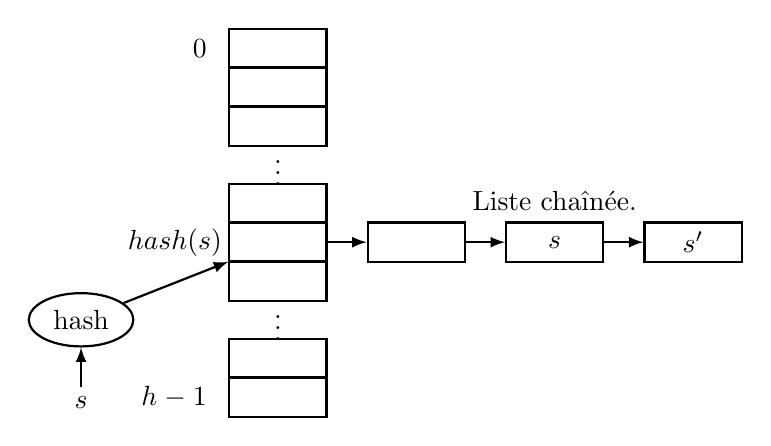
\begin{tikzpicture}[
          hashtable/.style={text width=1cm,minimum height=.5cm,node distance=14,align=center},
          hash/.style={draw,rectangle,hashtable},
          lab/.style={align=right,text width=1cm,node distance=40},
          list/.style={hash,node distance=50},
          every path/.style={draw,->,thick,>=latex}
        ]
        %hashtable
        \node[hash] (0) at (0,0) {};
        \node[below of = 0,hash] (1) {};
        \node[below of = 1,hash] (2) {};
        \node[below of = 2,hashtable] (3) {\vdots};
        \node[below of = 3,hash] (4) {};
        \node[below of = 4,hash] (5) {};
        \node[below of = 5,hash] (6) {};
        \node[below of = 6,hashtable] (7) {\vdots};
        \node[below of = 7,hash] (8) {};
        \node[below of = 8,hash] (9) {};

        %labels
        \node[left of = 0,lab] {$0$};
        \node[left of = 9,lab] {$h-1$};
        \node[left of = 5,lab] {$hash (s)$};

        %linked list
        \node[right of = 5,list] (51) {};
        \node[right of = 51,list] (52) {$s$};
        \node[right of = 52,list] (53) {$s'$};
        \path
        (5) edge (51)
        (51) edge (52)
        (52) edge (53)
        ;
        \node[above of = 52,node distance=15] {Liste chaînée.};

        %left part
        \node (s) at (-2.5,-4.5) {$s$};
        \node[above of = s,draw,ellipse,node distance=30] (hash) {hash};
        \path
        (s) edge (hash)
        (hash) edge (5)
        ;
    \end{tikzpicture}

    Une deuxième structure de données est utilisée afin de gérer la notion d'accès par scope de visibilité. Une liste de listes à ajout en tête est utilisée ici. Elle sera utilisée comme une pile. L'utilisation d'une pile n'est pas appropriée puisque dans de nombreux cas il sera intéressant de pouvoir parcourir la liste en profondeur. Or cela est coûteux avec une pile. Voici une illustration permettant de visualiser cette structure de données. (x, y, z et w représentent des noms de symbols donc de type String.)

    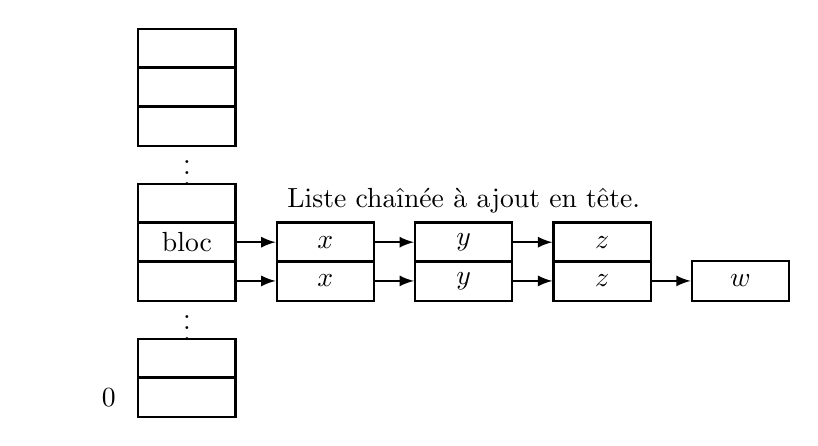
\begin{tikzpicture}[
          hashtable/.style={text width=1cm,minimum height=.5cm,node distance=14,align=center},
          hash/.style={draw,rectangle,hashtable},
          lab/.style={align=right,text width=1cm,node distance=40},
          list/.style={hash,node distance=50},
          every path/.style={draw,->,thick,>=latex}
        ]
        \node[hash] (0) at (0,0) {};
        \node[below of = 0,hash] (1) {};
        \node[below of = 1,hash] (2) {};
        \node[below of = 2,hashtable] (3) {\vdots};
        \node[below of = 3,hash] (4) {};
        \node[below of = 4,hash] (5) {bloc};
        \node[below of = 5,hash] (6) {};
        \node[below of = 6,hashtable] (7) {\vdots};
        \node[below of = 7,hash] (8) {};
        \node[below of = 8,hash] (9) {};

        %labels
        \node[left of = 0,lab] {};
        \node[left of = 9,lab] {$0$};
        \node[left of = 5,lab] {};

        %linked list
        \node[right of = 5,list] (51) {$x$};
        \node[right of = 51,list] (52) {$y$};
        \node[right of = 52,list] (53) {$z$};
        \path
        (5) edge (51)
        (51) edge (52)
        (52) edge (53)
        ;

        %linked list
        \node[right of = 6,list] (61) {$x$};
        \node[right of = 61,list] (62) {$y$};
        \node[right of = 62,list] (63) {$z$};
        \node[right of = 63,list] (64) {$w$};
        \path
        (6) edge (61)
        (61) edge (62)
        (62) edge (63)
        (63) edge (64)
        ;
        \node[above of = 52,node distance=15] {Liste chaînée à ajout en tête.};
        
        
    \end{tikzpicture}    
    \subsubsection{Comment fonctionne la pile avec la table de hachage ?}
      Les blocs sont imbriqués les uns dans les autres. Lorsque des déclarations sont faîtes dans des blocs imbriqués il arrive que des symboles masquent des symboles déclararés dans des blocs parents.\\
      Quand dans un bloc un symbol est utilisé il fait référence à la première déclaration qui en a été faite. C'est à ce niveau que la pile est importante.\\

      Les niveaux de la pile représentent les niveaux d'imbrications. Dans cette pile, chacuns des niveaux ont une liste de symboles. C'est symboles sont représentés par leurs noms. Ainsi, grâce à la table de hachage il est aisé de récupérer l'instance correspondant au symbol en question.\\

      Lors de l'analyse, lorsqu'un bloc a été entièrement analysé, les déclarations de symboles qui y ont été réalisés deviennent obsolètes pour la suite de l'analyse. Il est nécessaire de faire du nettoyage dans la pile.\\

      Cette étape consiste à dépiler le bloc courant de la pile. Pour ce faire, le symbol en tête de liste pointée par ce bloc (celui le plus haut dans la pile) est supprimé. Cela doit être répété afin de vider la liste. La suppression est rapide puisque qu'il suffit de supprimer la tete de liste à chaque fois.\\
      Une fois la liste vide, le bloc peut être dépilé.

  \subsection{Exemple d'analyse sur un programme simple}
    \begin{multicols}{2}
        
        \begin{minted}[bgcolor=bg-gray]{c}
        { // bloc 1
          int a = 2;
          int b = a + 1; // b=3
         { // bloc 2
           int a = b + 2; // a=5
           { // bloc 3
             int b = a + 3; // b=8
             int c = a + b; // c=13
           }
           int c = a + b; // c=8
         }
         int c = a + b; // c=5
        }

        \end{minted}

      \columnbreak
        Ce programme réalise différents appels et et différentes déclarations au sein de plusieurs blocs imbriqués. Nous remarquons également que certaines variables sont masquées. Les commentaires nous aides à comprendre l'effet que cela implique sur le programme puisque l'expression a + b n'a pas la même valeur en fonction du bloc dans lequel elle est évaluée. Car ils contiennent des déclarations de a et de b qui masquent les précédentes.\\

        Déroulons pas à pas l'analyse des symboles.
       
    \end{multicols}
    % step 1
    \subsubsection{Première étape}
    \begin{multicols}{2}
        
        \begin{minted}[bgcolor=bg-gray]{c}
        { // bloc 1 <-----
          int a = 2;
          int b = a + 1; // b=3
         { // bloc 2
           int a = b + 2; // a=5
           { // bloc 3
             int b = a + 3; // b=8
             int c = a + b; // c=13
           }
           int c = a + b; // c=8
         }
         int c = a + b; // c=5
        }

        \end{minted}

      \columnbreak
        L'analyse commence par le bloc 1. La table de hachage est vide et la pile également.
      \end{multicols}

      \begin{multicols}{2}
        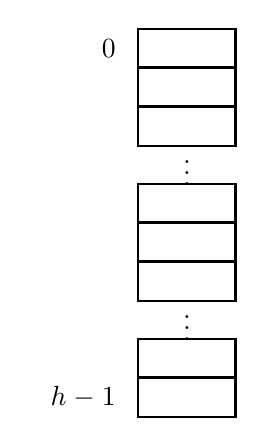
\begin{tikzpicture}[
            hashtable/.style={text width=1cm,minimum height=.5cm,node distance=14,align=center},
            hash/.style={draw,rectangle,hashtable},
            lab/.style={align=right,text width=1cm,node distance=40},
            list/.style={hash,node distance=50},
            every path/.style={draw,->,thick,>=latex}
          ]
          %hashtable
          \node[hash] (0) at (0,0) {};
          \node[below of = 0,hash] (1) {};
          \node[below of = 1,hash] (2) {};
          \node[below of = 2,hashtable] (3) {\vdots};
          \node[below of = 3,hash] (4) {};
          \node[below of = 4,hash] (5) {};
          \node[below of = 5,hash] (6) {};
          \node[below of = 6,hashtable] (7) {\vdots};
          \node[below of = 7,hash] (8) {};
          \node[below of = 8,hash] (9) {};

          %labels
          \node[left of = 0,lab] {$0$};
          \node[left of = 9,lab] {$h-1$};
      \end{tikzpicture}
      
      \columnbreak

      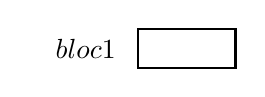
\begin{tikzpicture}[
            hashtable/.style={text width=1cm,minimum height=.5cm,node distance=14,align=center},
            hash/.style={draw,rectangle,hashtable},
            lab/.style={align=right,text width=1cm,node distance=40},
            list/.style={hash,node distance=50},
            every path/.style={draw,->,thick,>=latex}
          ]
          \node[hash] (0) at (0,0) {};
          
          %labels
          \node[left of = 0,lab] {$bloc 1$};
          
      \end{tikzpicture} 
    \end{multicols}

    % step 2
    \subsubsection{Deuxième étape}
    \begin{multicols}{2}
        
        \begin{minted}[bgcolor=bg-gray]{c}
        { // bloc 1
          int a = 2; <-----
          int b = a + 1; // b=3
         { // bloc 2
           int a = b + 2; // a=5
           { // bloc 3
             int b = a + 3; // b=8
             int c = a + b; // c=13
           }
           int c = a + b; // c=8
         }
         int c = a + b; // c=5
        }

        \end{minted}

      \columnbreak
        Bloc 1:\\
        Déclaration de variable: int a = 2;\\
        La pile est vide donc on doit créer le symbol dans la table.
      \end{multicols}

      \begin{multicols}{2}
        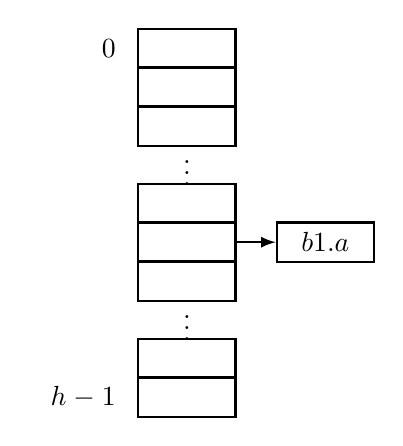
\begin{tikzpicture}[
            hashtable/.style={text width=1cm,minimum height=.5cm,node distance=14,align=center},
            hash/.style={draw,rectangle,hashtable},
            lab/.style={align=right,text width=1cm,node distance=40},
            list/.style={hash,node distance=50},
            every path/.style={draw,->,thick,>=latex}
          ]
          %hashtable
          \node[hash] (0) at (0,0) {};
          \node[below of = 0,hash] (1) {};
          \node[below of = 1,hash] (2) {};
          \node[below of = 2,hashtable] (3) {\vdots};
          \node[below of = 3,hash] (4) {};
          \node[below of = 4,hash] (5) {};
          \node[below of = 5,hash] (6) {};
          \node[below of = 6,hashtable] (7) {\vdots};
          \node[below of = 7,hash] (8) {};
          \node[below of = 8,hash] (9) {};

          %labels
          \node[left of = 0,lab] {$0$};
          \node[left of = 9,lab] {$h-1$};

          %linked list
          \node[right of = 5,list] (51) {$b1.a$};
          \path
          (5) edge (51)
          ;

      \end{tikzpicture}
      
      \columnbreak
      
      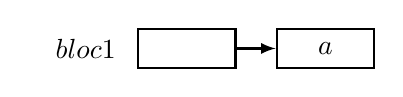
\begin{tikzpicture}[
            hashtable/.style={text width=1cm,minimum height=.5cm,node distance=14,align=center},
            hash/.style={draw,rectangle,hashtable},
            lab/.style={align=right,text width=1cm,node distance=40},
            list/.style={hash,node distance=50},
            every path/.style={draw,->,thick,>=latex}
          ]
          \node[hash] (0) at (0,0) {};
          
          %labels
          \node[left of = 0,lab] {$bloc 1$};

          %linked list
          \node[right of = 0,list] (01) {$a$};
          \path
          (0) edge (01)
          ;
          
      \end{tikzpicture} 
    \end{multicols}

    % step 3
    \subsubsection{Troisième étape}
    \begin{multicols}{2}
        
        \begin{minted}[bgcolor=bg-gray]{c}
        { // bloc 1
          int a = 2;
          int b = a + 1; // b=3 <-----
         { // bloc 2
           int a = b + 2; // a=5
           { // bloc 3
             int b = a + 3; // b=8
             int c = a + b; // c=13
           }
           int c = a + b; // c=8
         }
         int c = a + b; // c=5
        }

        \end{minted}

      \columnbreak
        Bloc 1:\\
        Déclaration de variable: int b = a + 1;\\
        La pile n'est pas vide donc on cherche la définition du symbol a.\\
        On commence par le haut de la pile et on parcours la liste.\\
        Le symbol est trouvé donc il n'y a pas d'erreur de sémantique.\\
        Le symbol b peut être créé.
      \end{multicols}

      \begin{multicols}{2}
        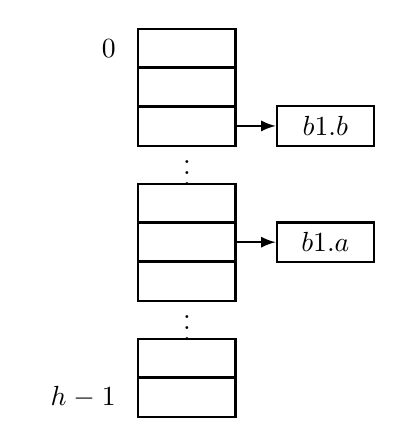
\begin{tikzpicture}[
            hashtable/.style={text width=1cm,minimum height=.5cm,node distance=14,align=center},
            hash/.style={draw,rectangle,hashtable},
            lab/.style={align=right,text width=1cm,node distance=40},
            list/.style={hash,node distance=50},
            every path/.style={draw,->,thick,>=latex}
          ]
          %hashtable
          \node[hash] (0) at (0,0) {};
          \node[below of = 0,hash] (1) {};
          \node[below of = 1,hash] (2) {};
          \node[below of = 2,hashtable] (3) {\vdots};
          \node[below of = 3,hash] (4) {};
          \node[below of = 4,hash] (5) {};
          \node[below of = 5,hash] (6) {};
          \node[below of = 6,hashtable] (7) {\vdots};
          \node[below of = 7,hash] (8) {};
          \node[below of = 8,hash] (9) {};

          %labels
          \node[left of = 0,lab] {$0$};
          \node[left of = 9,lab] {$h-1$};

          %linked list
          \node[right of = 5,list] (51) {$b1.a$};
          \node[right of = 2,list] (21) {$b1.b$};
          \path
          (5) edge (51)
          (2) edge (21)
          ;

      \end{tikzpicture}
      
      \columnbreak
      
      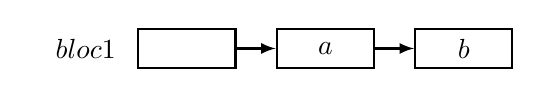
\begin{tikzpicture}[
            hashtable/.style={text width=1cm,minimum height=.5cm,node distance=14,align=center},
            hash/.style={draw,rectangle,hashtable},
            lab/.style={align=right,text width=1cm,node distance=40},
            list/.style={hash,node distance=50},
            every path/.style={draw,->,thick,>=latex}
          ]
          \node[hash] (0) at (0,0) {};
          
          %labels
          \node[left of = 0,lab] {$bloc 1$};

          %linked list
          \node[right of = 0,list] (01) {$a$};
          \node[right of = 01,list] (02) {$b$};
          \path
          (0) edge (01)
          (01) edge (02)
          ;
          
      \end{tikzpicture} 
    \end{multicols}

    % step 4
    \subsubsection{Quatrième étape}
    \begin{multicols}{2}
        
        \begin{minted}[bgcolor=bg-gray]{c}
        { // bloc 1
          int a = 2;
          int b = a + 1; // b=3
         { // bloc 2 <-----
           int a = b + 2; // a=5
           { // bloc 3
             int b = a + 3; // b=8
             int c = a + b; // c=13
           }
           int c = a + b; // c=8
         }
         int c = a + b; // c=5
        }

        \end{minted}

      \columnbreak
        Bloc 2: Création d'une liste vide sur la pile
        
      \end{multicols}

      \begin{multicols}{2}
        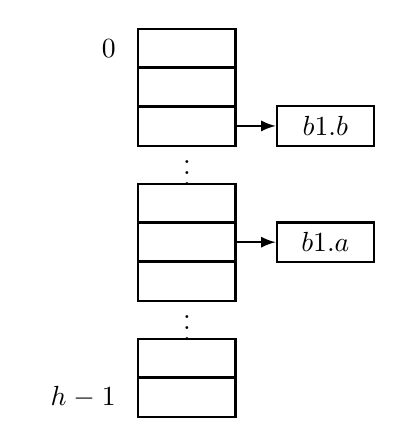
\begin{tikzpicture}[
            hashtable/.style={text width=1cm,minimum height=.5cm,node distance=14,align=center},
            hash/.style={draw,rectangle,hashtable},
            lab/.style={align=right,text width=1cm,node distance=40},
            list/.style={hash,node distance=50},
            every path/.style={draw,->,thick,>=latex}
          ]
          %hashtable
          \node[hash] (0) at (0,0) {};
          \node[below of = 0,hash] (1) {};
          \node[below of = 1,hash] (2) {};
          \node[below of = 2,hashtable] (3) {\vdots};
          \node[below of = 3,hash] (4) {};
          \node[below of = 4,hash] (5) {};
          \node[below of = 5,hash] (6) {};
          \node[below of = 6,hashtable] (7) {\vdots};
          \node[below of = 7,hash] (8) {};
          \node[below of = 8,hash] (9) {};

          %labels
          \node[left of = 0,lab] {$0$};
          \node[left of = 9,lab] {$h-1$};

          %linked list
          \node[right of = 5,list] (51) {$b1.a$};
          \node[right of = 2,list] (21) {$b1.b$};
          \path
          (5) edge (51)
          (2) edge (21)
          ;

      \end{tikzpicture}
      
      \columnbreak
      
      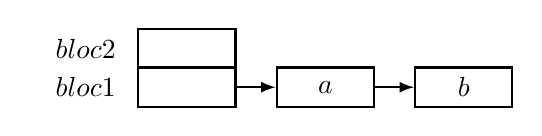
\begin{tikzpicture}[
            hashtable/.style={text width=1cm,minimum height=.5cm,node distance=14,align=center},
            hash/.style={draw,rectangle,hashtable},
            lab/.style={align=right,text width=1cm,node distance=40},
            list/.style={hash,node distance=50},
            every path/.style={draw,->,thick,>=latex}
          ]
          \node[hash] (1) at (0,0) {};
          \node[below of = 1,hash] (0) {};
          
          %labels
          \node[left of = 0,lab] {$bloc 1$};
          \node[left of = 1,lab] {$bloc 2$};

          %linked list
          \node[right of = 0,list] (01) {$a$};
          \node[right of = 01,list] (02) {$b$};
          \path
          (0) edge (01)
          (01) edge (02)
          ;
          
      \end{tikzpicture} 
    \end{multicols}

    % step 5
    \subsubsection{Cinquième étape}
    \begin{multicols}{2}
        
        \begin{minted}[bgcolor=bg-gray]{c}
        { // bloc 1
          int a = 2;
          int b = a + 1; // b=3
         { // bloc 2
           int a = b + 2; // a=5 <-----
           { // bloc 3
             int b = a + 3; // b=8
             int c = a + b; // c=13
           }
           int c = a + b; // c=8
         }
         int c = a + b; // c=5
        }

        \end{minted}

      \columnbreak
        Bloc 2:\\
        Déclaration de variable: int a = b + 2;\\
        La pile n'est pas vide donc on cherche la définition du symbol b.\\
        On commence par le haut de la pile et on parcours la liste.\\
        La liste est vide donc on recherche dans le bloc suivant immédiatement plus bas que le bloc courant.\\
        Le symbol est trouvé donc il n'y a pas d'erreur de sémantique.\\
        Le symbol a peut être créé.
        
      \end{multicols}

      \begin{multicols}{2}
        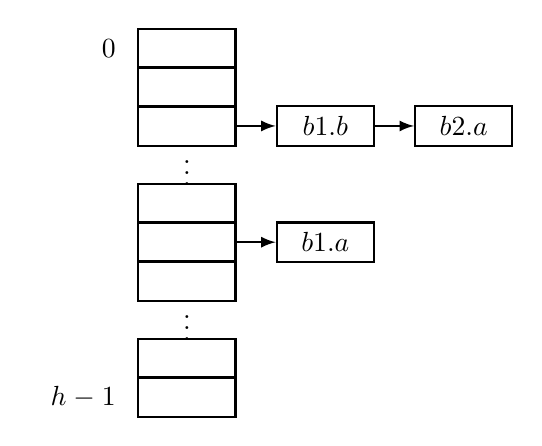
\begin{tikzpicture}[
            hashtable/.style={text width=1cm,minimum height=.5cm,node distance=14,align=center},
            hash/.style={draw,rectangle,hashtable},
            lab/.style={align=right,text width=1cm,node distance=40},
            list/.style={hash,node distance=50},
            every path/.style={draw,->,thick,>=latex}
          ]
          %hashtable
          \node[hash] (0) at (0,0) {};
          \node[below of = 0,hash] (1) {};
          \node[below of = 1,hash] (2) {};
          \node[below of = 2,hashtable] (3) {\vdots};
          \node[below of = 3,hash] (4) {};
          \node[below of = 4,hash] (5) {};
          \node[below of = 5,hash] (6) {};
          \node[below of = 6,hashtable] (7) {\vdots};
          \node[below of = 7,hash] (8) {};
          \node[below of = 8,hash] (9) {};

          %labels
          \node[left of = 0,lab] {$0$};
          \node[left of = 9,lab] {$h-1$};

          %linked list
          \node[right of = 5,list] (51) {$b1.a$};
          \node[right of = 2,list] (21) {$b1.b$};
          \node[right of = 21,list] (22) {$b2.a$};
          \path
          (5) edge (51)
          (2) edge (21)
          (21) edge (22)
          ;

      \end{tikzpicture}
      
      \columnbreak
      
      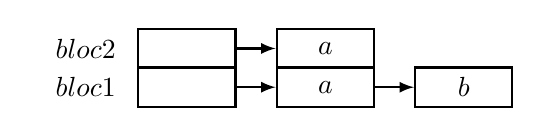
\begin{tikzpicture}[
            hashtable/.style={text width=1cm,minimum height=.5cm,node distance=14,align=center},
            hash/.style={draw,rectangle,hashtable},
            lab/.style={align=right,text width=1cm,node distance=40},
            list/.style={hash,node distance=50},
            every path/.style={draw,->,thick,>=latex}
          ]
          \node[hash] (1) at (0,0) {};
          \node[below of = 1,hash] (0) {};
          
          %labels
          \node[left of = 0,lab] {$bloc 1$};
          \node[left of = 1,lab] {$bloc 2$};

          %linked list
          \node[right of = 0,list] (01) {$a$};
          \node[right of = 01,list] (02) {$b$};
          \node[right of = 1,list] (11) {$a$};
          \path
          (0) edge (01)
          (01) edge (02)
          (1) edge (11)
          ;
          
      \end{tikzpicture} 
    \end{multicols}

    %%%%%%%
    %% TODO : Revoir le fonctionnement de la table de hachage avec la pile
    %%        Cela me semble confus..
    %%%%%%%

 \section{Interface de la table des symboles}
    \begin{minted}[bgcolor=bg-gray]{cpp}
    /**
     * Interface ITableOfSymbol.
     * Specifie les operations sur la table des symboles.
     */
    class ITableOfSymbol{public:
      // Requete

      /**
       * Retourne l'instance representant le symbol en fonction de son nom.
       * @param sym Nom du symbol.
       */
      virtual SemanticPtr* getSymbol(String sym) = 0;

      // Commandes

      /**
       * Place le curseur interne sur un nouveau bloc.
       * Toutes les futures operations se feront sur ce bloc.
       */
      virtual void enterBloc() = 0;

      /**
       * Deplace le curseur interne sur le bloc precedent.
       * Toutes les futures operations se feront sur ce bloc.
       */
      virtual void exitBloc() = 0;

      /**
       * Ajoute une definition de symbol dans la table des symboles.
       * @param sym Nom du symbol
       * @param sptr pointeur sur l'instance qui represente le symbol.
       */
      virtual void addSymbol(String sym, SemanticPtr* sptr) = 0;
    }
    \end{minted}

  \subsection{enterBloc}
    La fonction enterBloc doit être appellée lorsque l'analyseur sémantique entre dans un bloc. Ainsi un nouveau bloc sera empilé sur la pile. Les recherches de symboles se feront en prenant en compte les niveaux d'imbrications des blocs.
  \subsection{exitBloc}
   Réciproquement, lorsque l'analyseur sémantique quitte un bloc, la fonction exitBloc doit être appellée. Cela permet de dépiler un bloc de la pile afin de supprimer les déclarations qui sont obsolètes car innaccessibles depuis l'exterieur du bloc.
\end{document}
